\chapter{Background}
\label{chap:background}

This chapter is organized into three sections. The first section provides an overview of the current layered and heterogeneous infrastructure
defined by the could-edge interplay. The second section describes the problem of the deployment independence of the applications by giving an
overview of the actual frameworks and methodologies. Finally, the third section describes the pulverization methodology in aggregate computing and
cyber-physical systems.

\section{Layered and heterogeneous infrastructure}
\label{sec:layered-heterogeneous-infrastructure}

\subsection{Cloud Fog and Edge interplay}
\label{sec:cloud-fog-edge-interplay}

% - New section ---------------------------------------------------------------

\section{Deployment independence}
\label{sec:deployment-independence}

The advantages of integrating different computing paradigms, such as cloud and edge computing, have already been acknowledged by numerous
industry and academia-based initiatives, one example is the OpenFog Consortium~\cite{opc}.

The cloud-edge computing integration is an open research topic since each of the two paradigms has its own use cases and advantages. The cloud
computing paradigm is well suited for large-scale applications that require high computational power and storage capacity. On the other hand, edge
computing is well suited for applications that require low latency and high reliability, such as autonomous vehicles, smart cities, and industrial
automation. The integration of the two paradigms can provide a more flexible and efficient solution for a wide range of applications.
Nevertheless, the integration of the two paradigms is not trivial, and different approaches can be used to tackle this problem.

In this context, we refer to ``deployment independence'' as the ability of an application to be deployed on any computing infrastructure by
separating the business logic from deployment and infrastructure aspects. In this way, the system logic can be developed without considering the
underlying infrastructure, since they are orthogonal aspects. This approach, on the one hand, allows for better-engineered systems where aspects of
development and deployment are separated; while on the other hand, one can make the best use of the available infrastructure according to the
dynamics of the system.

The following section will review the main methodologies that are in the literature and aspire to develop systems that integrate cloud-edge
infrastructure.

\subsection{Actual frameworks and methodologies}
\label{sec:actual-frameworks-methodologies}

Many frameworks and methodologies have been proposed in the literature to handle the edge-cloud continuum problem. The different approaches
proposed vary in complexity and use cases, each trying to solve a specific problem.

Among the methodologies and frameworks worth mentioning is osmotic computing which operates in the IoT environment focusing on a three-tier
architecture by leveraging microservices that can be moved around the infrastructure and frameworks such as DR-BIP and DReAM that are based on the
concept of "motif" and interaction rules and reconfiguration rules to manage system deployment.

The following is an overview of how these two methodologies work, highlighting their main features and how they try to solve the integration problem.

\subsubsection{Osmotic computing}

Osmotic computing~\cite{8781958} utilizes a concept known as a MEL (microelement) to encompass resources, services, and data. In the realm of IoT,
MELs can be structured as a graph and relocated across various infrastructures based on factors such as cost, security, privacy, and performance.
MELs encapsulate four distinct elements: microservices that provide specific functionality, microdata representing the flow of information to and from
sensors or actuators, microcomputing that performs various computational tasks using real-time and historic data, and microactuators that control the
state of physical resources using actuators at the network edge.

Each application can be decomposed into (cooperative) subprograms to improve deployability and scalability. This decomposition, in osmotic computing,
defines several interacting MELs, which are atomic entities providing simple functionalities. A graph of MELs can include several microservices
(MS) and microdata (MD) combined to provide a specific behavior. In osmosis, containers (or virtual components) are used to deploy dynamically and
support the migration of MELs across heterogeneous systems.

In osmotic computing, the computing environment is divided into three layers: cloud data centers (L1), edge systems and micro data centers (L2), and
IoT devices (L3).
At L3, the IoT devices capture raw data from the environment at a fixed frequency or by events. The L2 layer is composed of network devices such as
routers, switches and gateways, supported by protocols like \emph{OpenFlow} or hardware that enables network components to be accessed remotely.
Finally, L1 is composed of data centers, which are large-scale computing facilities that provide a large number of computing resources and storage
capacity.
The L2 layer can collect the data coming from devices at L3 enabling the collection of raw data and performing some computations before transferring
these data to L1.

Osmotic computing is an extension of elastic resource management, in which the deployment and migration strategies of microelements (MELs) can change
over time based on changing infrastructure and application requirements. Osmotic computing automates the configuration and reconfiguration of MELs
based on factors such as quality of service, security, and runtime perturbations.

The purpose of an osmotic platform is to balance the needs of both the infrastructure and the applications by automatically relocating microservices
to appropriate deployment locations. This approach focuses mainly on systems that are centrally managed and coordinated.

\begin{figure}
	\centering
	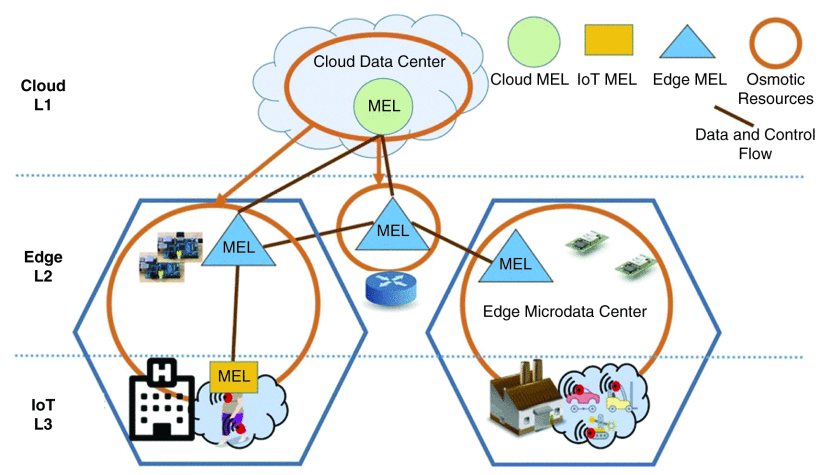
\includegraphics[width=0.8\linewidth]{figures/osmotic-architecture.png}
	\caption{Osmotic computing architecture reference.}
	\label{fig:osmotic-computing}
\end{figure}

\subsubsection{DR-BIP and DReAM framework}

The \emph{Dynamic Reconfigurable BIP} framework (DR-BIP)~\cite{10.1007/978-3-030-03424-5_20} includes three main aspects of dynamism: (I) the ability
to describe parametric system coordination for an arbitrary number of instances of component types, (II) the ability to add/delete components and
manage their interaction rules depending on dynamically changing conditions, and (III) allow services to seamlessly continue their activity on any
available device or computer (fluid architectures~\cite{taivalsaari2014liquid}).
The \emph{DR-BIP} framework is an extension of the \emph{Behavioral Interconnection Protocol} (BIP)~\cite{5719588} and
\emph{Dy-BIP} (a former extension that support dynamic interactions)~\cite{10.1007/978-3-642-30564-1_1}.

The DR-DIP framework provides support for runtime changes in the system, including component creation and removal, migration between motifs, and both
programmed and triggered reconfiguration.
The use of motifs allows components to interact with others based on their behavior and interaction rules within their new
motif, providing a flexible framework for coordination. The platform shares similarities with DReAM~\cite{de2020dream}, but the use of constraints
allows for more expressive coordination.

DR-BIP uses motifs as the basic unit for describing dynamic architectures (see~\Cref{fig:motif-concept}). Each motif includes the behavior of
components, the rules for interaction between components, and the rules for reconfiguring the motif, including adding, removing, or moving components.
Motifs are structurally organized as the deployment of component instances on a logical map.
Maps are arbitrary graph-like structures consisting of interconnected positions. Deployments relate components to positions on the map.
The definition of the motif is completed by two sets of rules: (I) the interaction rules, which define the behavior of the components and the
interaction between them, and (II) the reconfiguration rules, which define the conditions under which the motif can be reconfigured.

Systems are defined as collections of motif instances, each of which can evolve independently or in coordination with other motifs through shared
components or inter-motif reconfiguration rules. Inter-motif reconfiguration rules also allow for the creation and deletion of motif instances and
the exchange of components between motifs.

DR-BIP's behavior in a motif-based system is defined in a compositional way, where every motif has its own set of interactions determined by its
local structure. These interactions remain constant until the motif executes a reconfiguration action. In the absence of reconfigurations, the system
maintains a fixed architecture and operates like a normal BIP system. Interactions do not affect the architecture, while system and/or motif
reconfigurations change the architecture, but do not impact components, meaning running components retain their state, even though new components may
be added or removed.

\begin{figure}
	\centering
	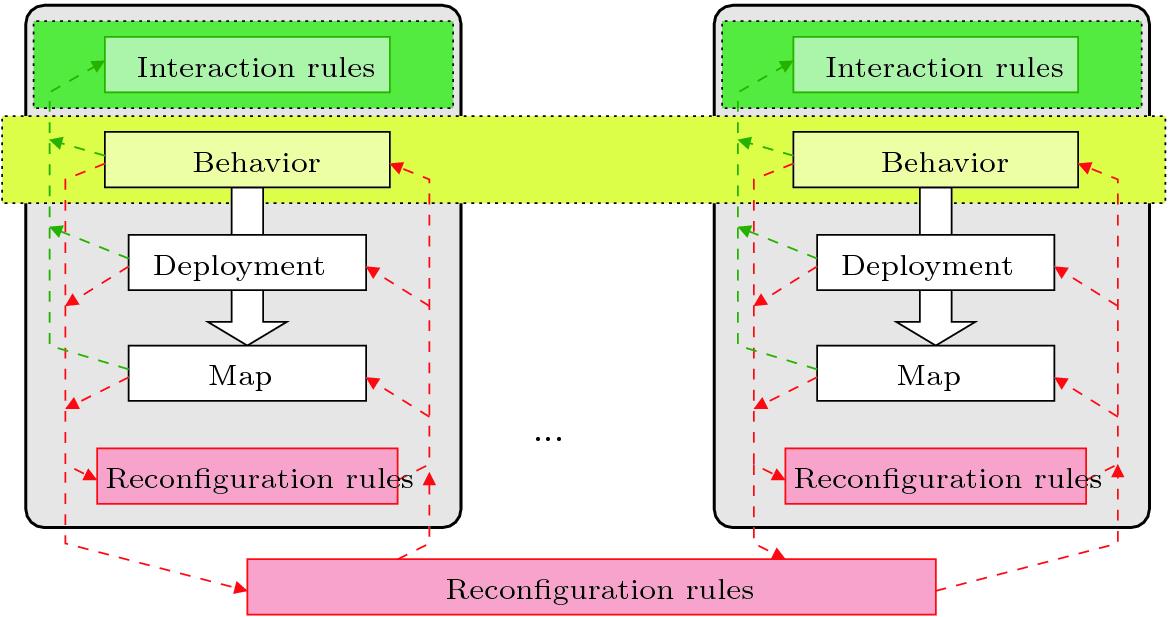
\includegraphics[width=0.8\linewidth]{figures/motif-concept.png}
	\caption{Motif-based System Concept.}
	\label{fig:motif-concept}
\end{figure}

% - New section ---------------------------------------------------------------

\section{Pulverization in Aggregate Computing and Cyber-Physical Systems}
\label{sec:pulverization-aggregate-computing-cps}
